\documentclass[a4paper,10pt,oneside]{book}
\usepackage[dutch]{babel}
\usepackage{amsmath}
\usepackage{amsfonts}
\usepackage{amssymb}
\usepackage{amsthm}
\usepackage{subfiles}
\usepackage{enumerate}
\usepackage{float}
\usepackage{url}
\usepackage[final]{pdfpages}

\setlength{\textwidth}{6in} 
\addtolength{\hoffset}{-0.5in}
\setlength{\topmargin}{-0.2in}
\setlength{\textheight}{9in}

\makeatletter
\renewcommand*\env@matrix[1][*\c@MaxMatrixCols c]{%
  \hskip -\arraycolsep
  \let\@ifnextchar\new@ifnextchar
  \array{#1}}
\makeatother


\date{2013-2014}

\begin{document}

%----------------------------------------------------------------------------------------
%	TITLE PAGE
%----------------------------------------------------------------------------------------

\begin{titlepage}
\hbox{
\hspace*{0.2\textwidth}
\rule{1pt}{\textheight}
\rule{2pt}{\textheight}
\rule{3pt}{\textheight}
\rule{4pt}{\textheight}
\rule{5pt}{\textheight}
\hspace*{0.05\textwidth}
\parbox[b]{0.75\textwidth}
{
{\noindent\Huge\bfseries Lineaire Algebra}\\[2\baselineskip]

{\huge \textsc{Tom Sydney Kerckhove}}\\\\\\
{Met dank aan}\\\\
{\Large \textsc{Ward Schodts}}\\\\
{\large \textsc{Nicholas Haesen}}\\
{\large \textsc{Thomas Dierckx}}\\
{\large \textsc{Frederik Goovaerts}}\\
{\large \textsc{Jorik De Waen}}\\
{\large \textsc{Egon Okerman}}\\\\\\



{\small Versie 0.0.1.32}



\vspace{0.5\textheight} % Whitespace
}
}
\end{titlepage}

\subfile{inleiding}

\newpage
\tableofcontents
\pagebreak


\part{Theorie}
\subfile{hoofdstuk_1_theorie}
\subfile{hoofdstuk_2_theorie}
\subfile{hoofdstuk_3_theorie}
\subfile{hoofdstuk_4_theorie}
\subfile{hoofdstuk_5_theorie}
\subfile{hoofdstuk_6_theorie}

\part{Oefeningen}
\subfile{hoofdstuk_1_oefeningen}
\subfile{hoofdstuk_2_oefeningen}
\subfile{hoofdstuk_3_oefeningen}
\subfile{hoofdstuk_4_oefeningen}
\subfile{hoofdstuk_5_oefeningen}
\subfile{hoofdstuk_6_oefeningen}

\part{Extra}
\subfile{tipsntricks}

\chapter{Zelfreflecties}
\subfile{zelfreflectie_1}
\subfile{zelfreflectie_2}
\subfile{zelfreflectie_3}
\subfile{zelfreflectie_4}
\subfile{zelfreflectie_5}
\subfile{zelfreflectie_6}

\chapter{Huistaken}
\subfile{huistaak_1}
\subfile{huistaak_2}

\appendix
\chapter{Errata van de curus}
\subfile{errata}

\chapter{Opgaven}
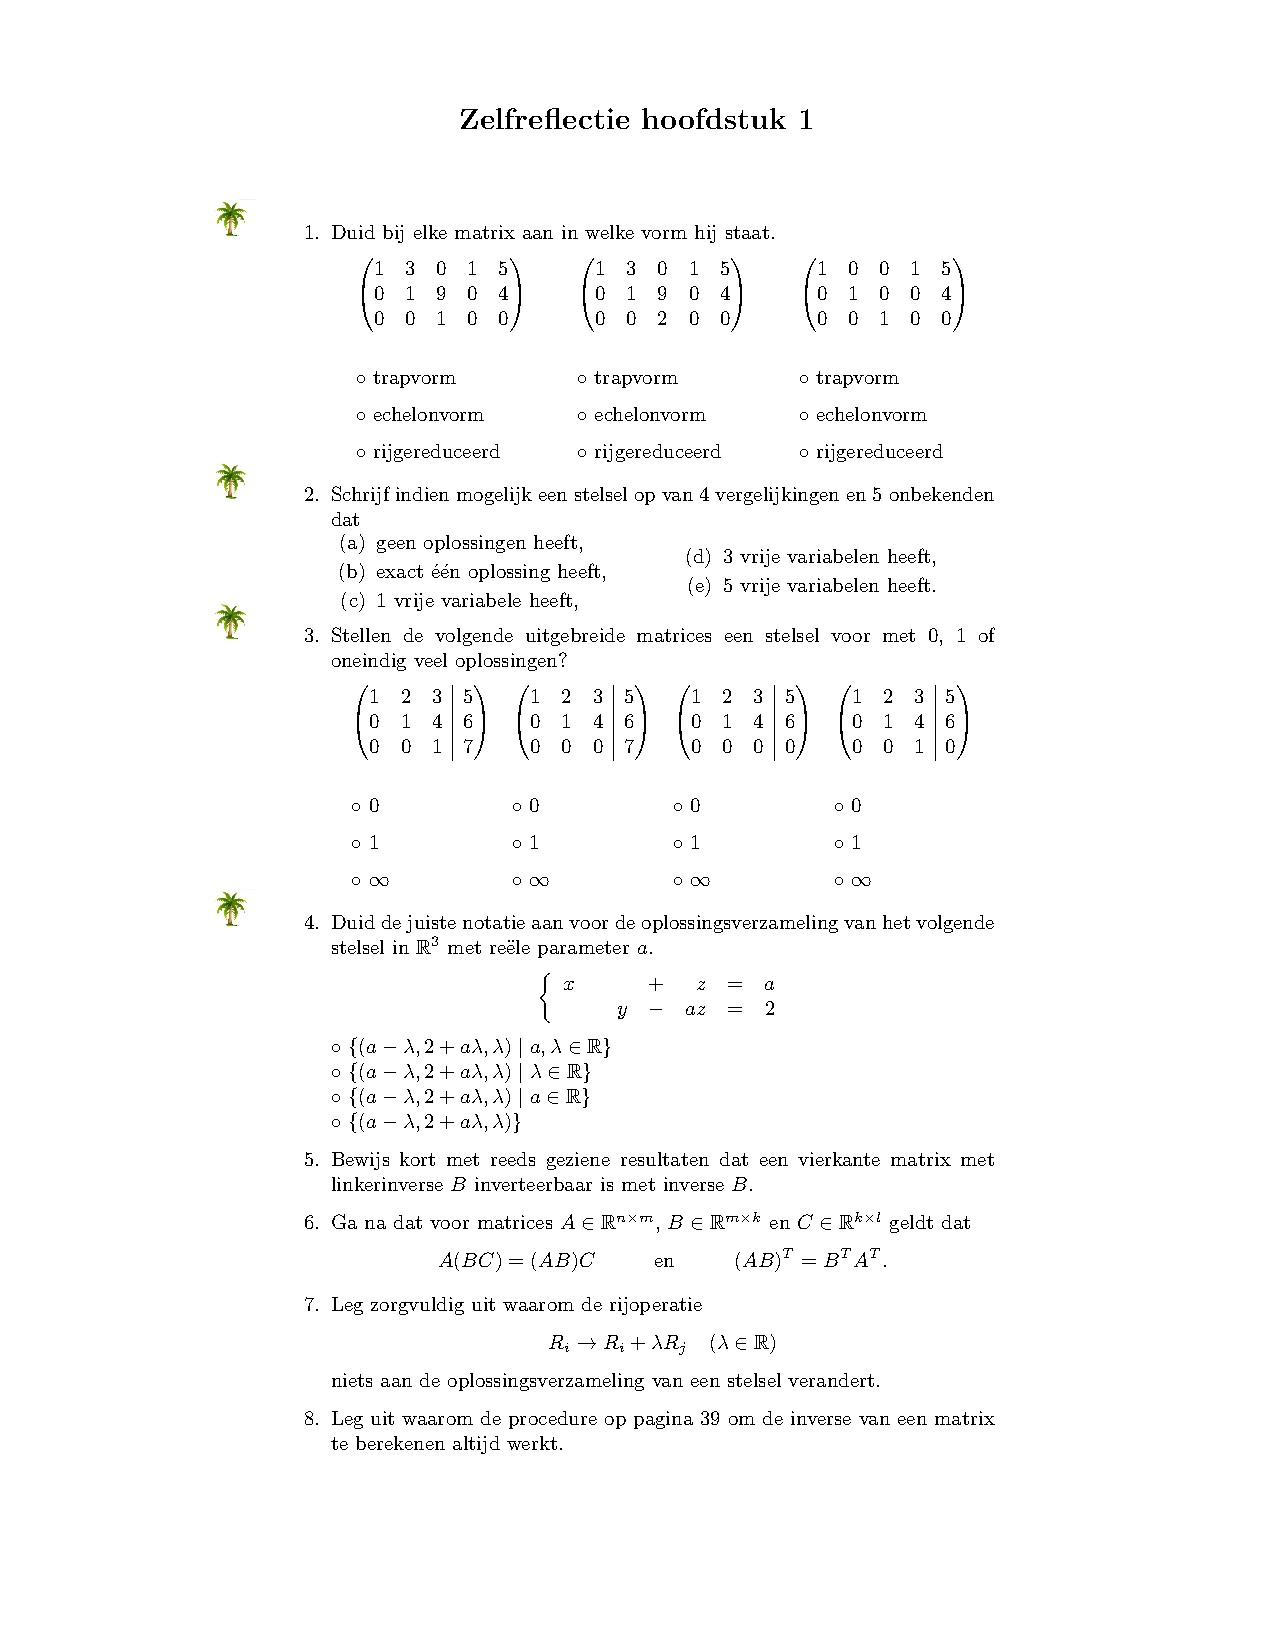
\includepdf[pages=-]{opgaven/zelfreflectie_H1.pdf}
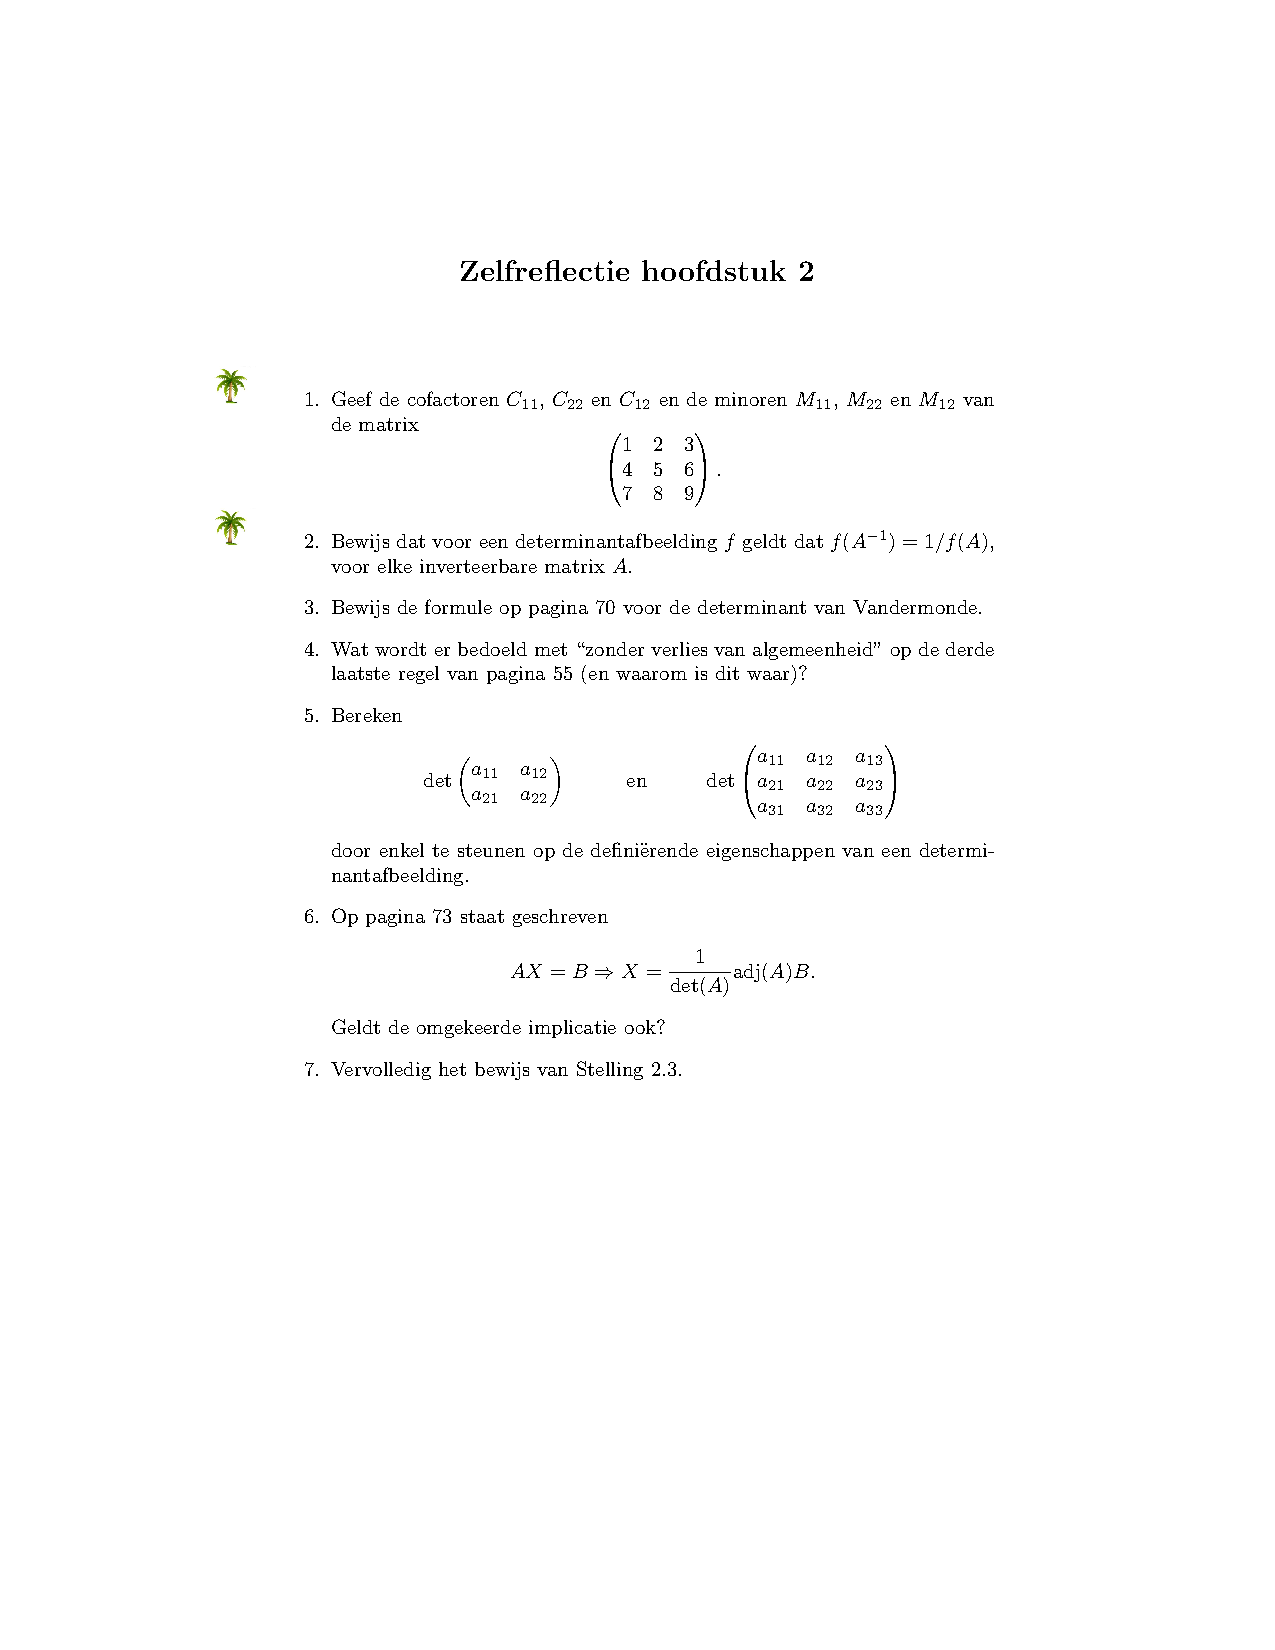
\includepdf[pages=-]{opgaven/zelfreflectie_H2.pdf}
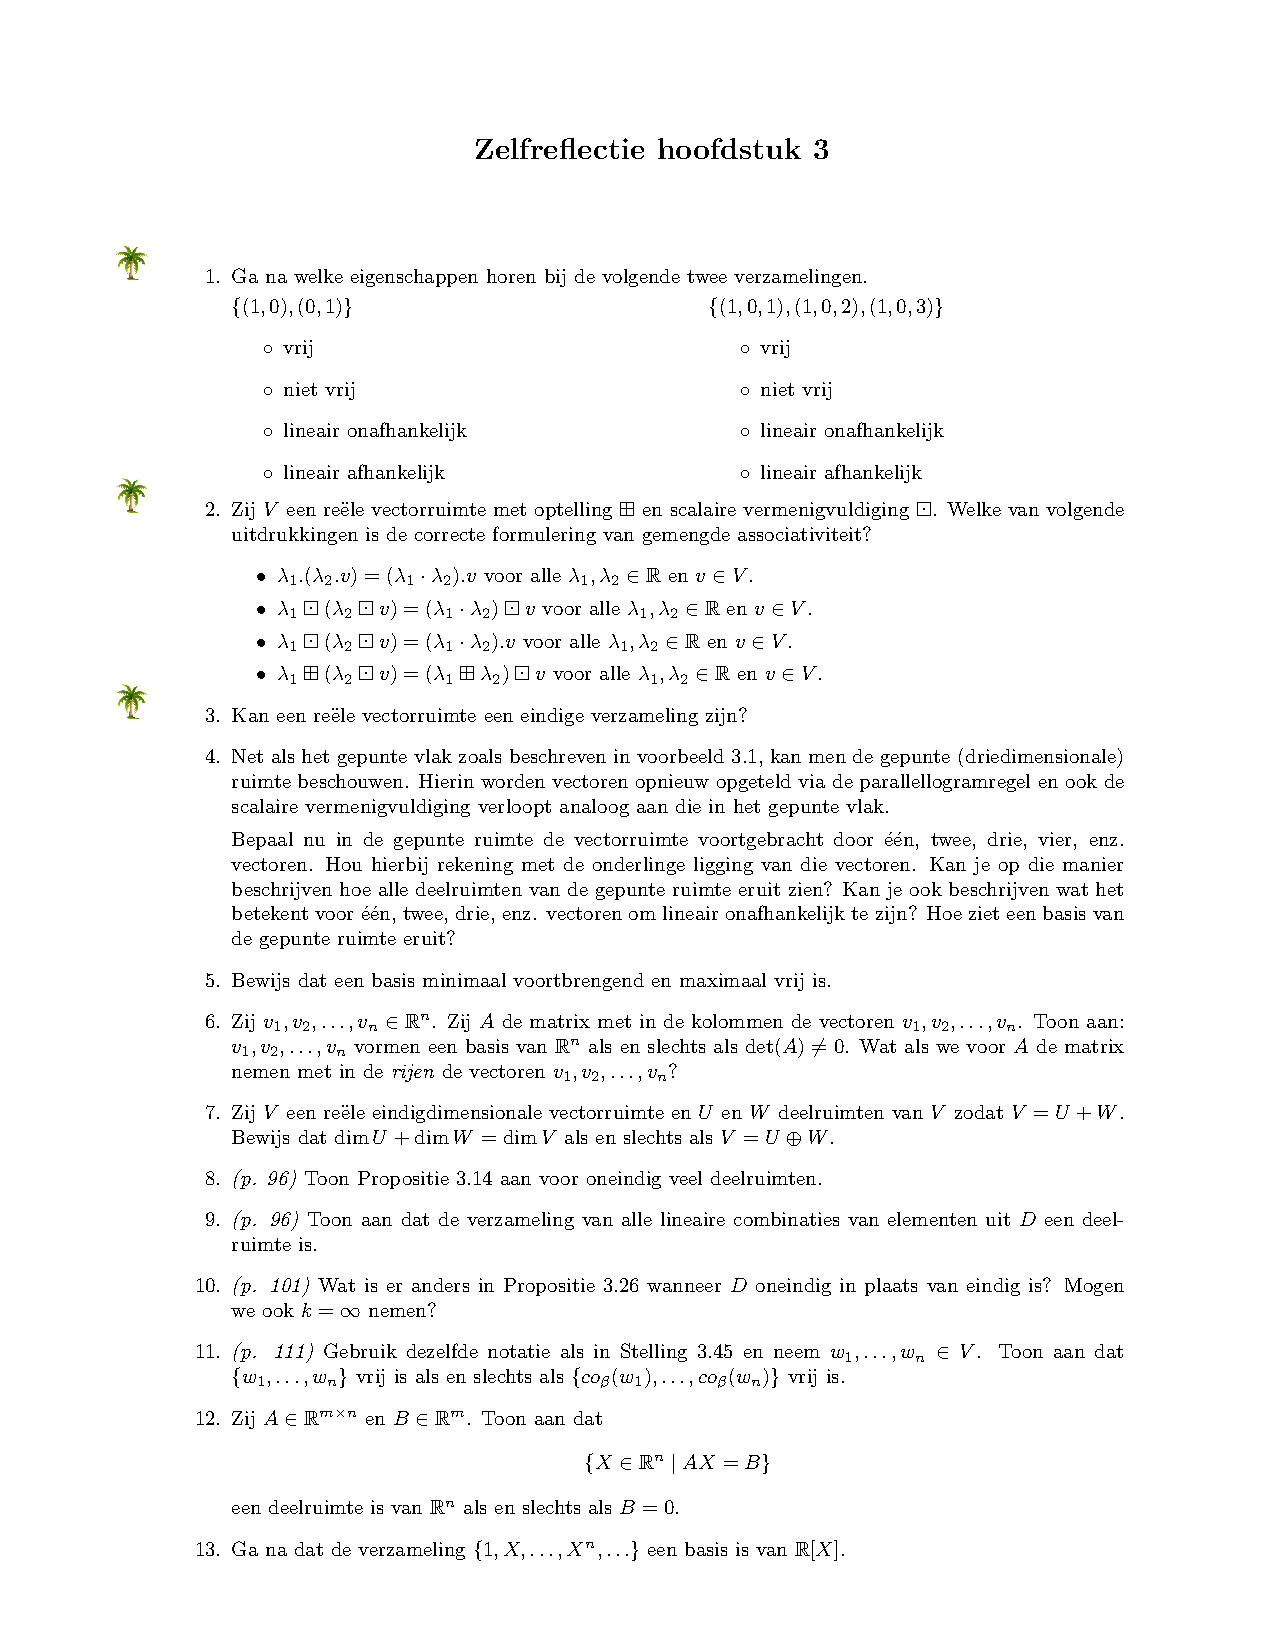
\includepdf[pages=-]{opgaven/zelfreflectie_H3.pdf}
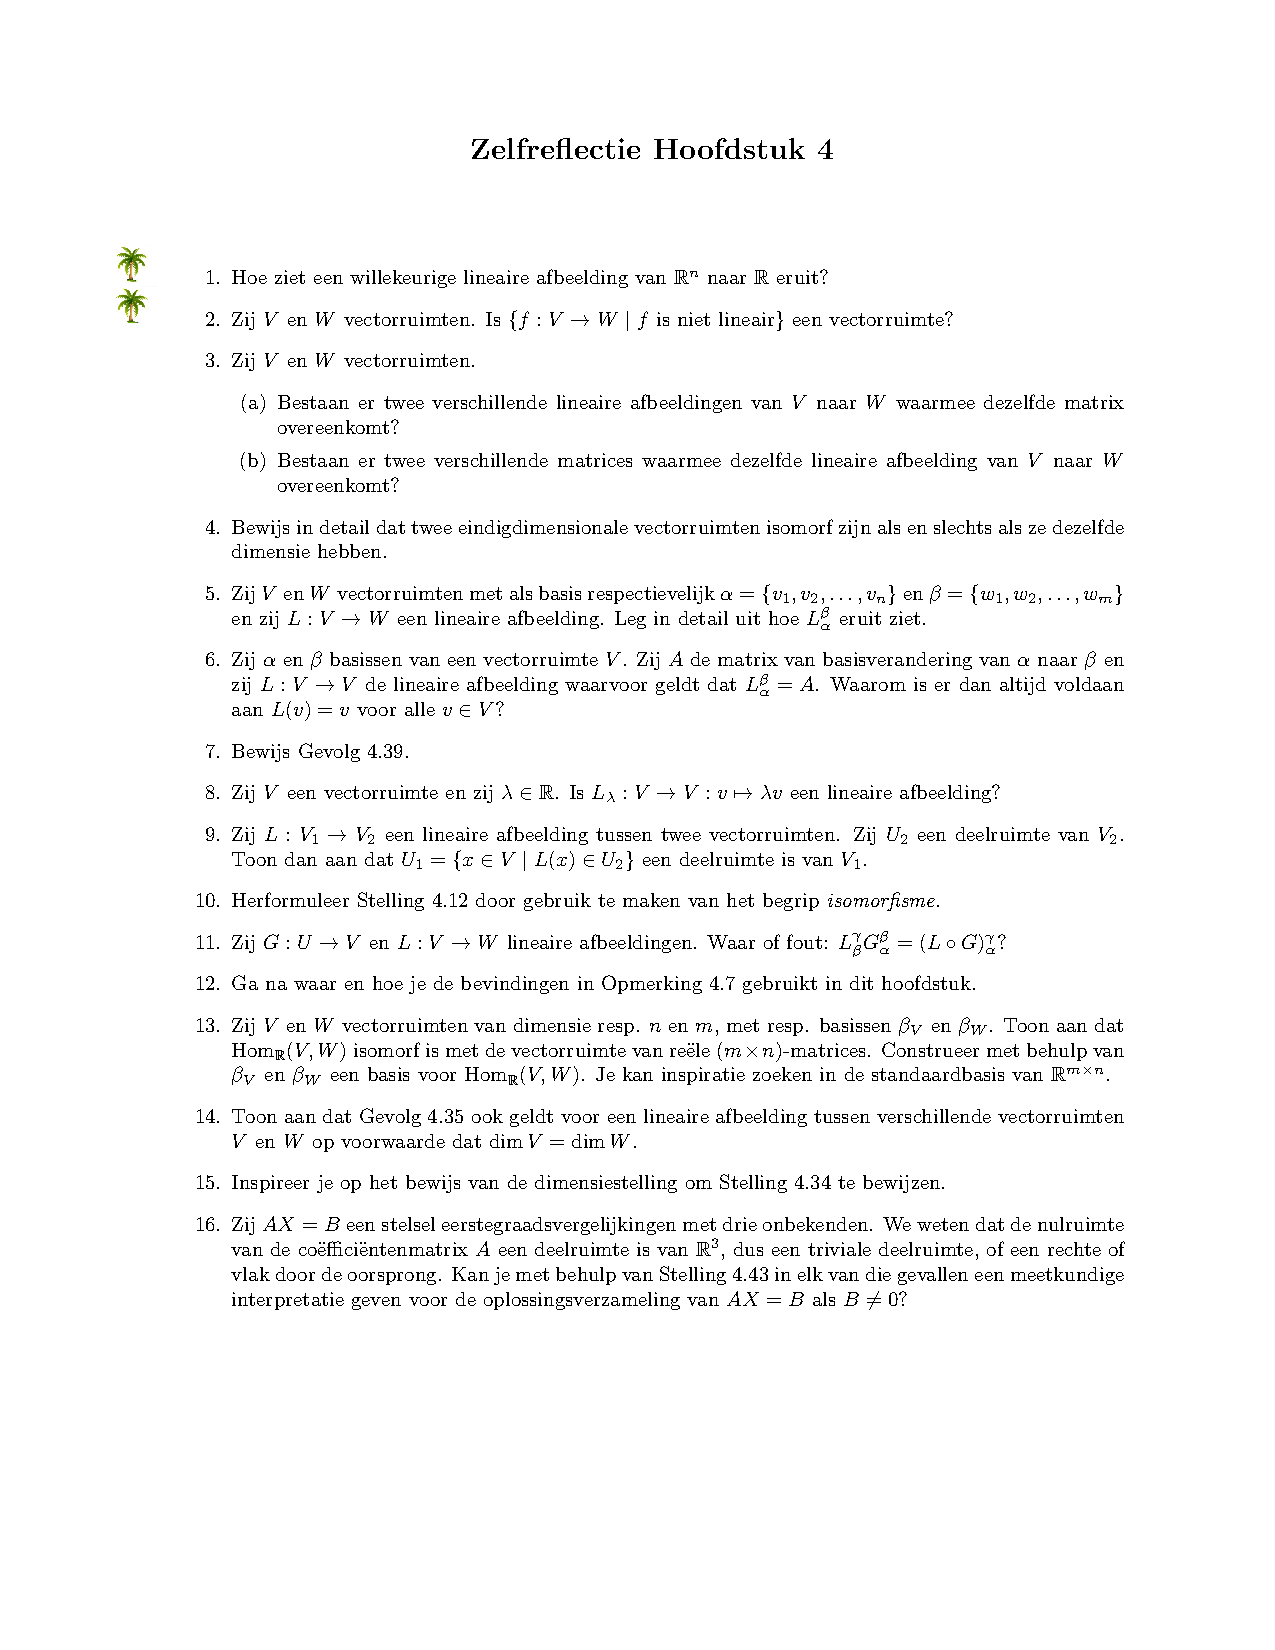
\includepdf[pages=-]{opgaven/zelfreflectie_H4.pdf}
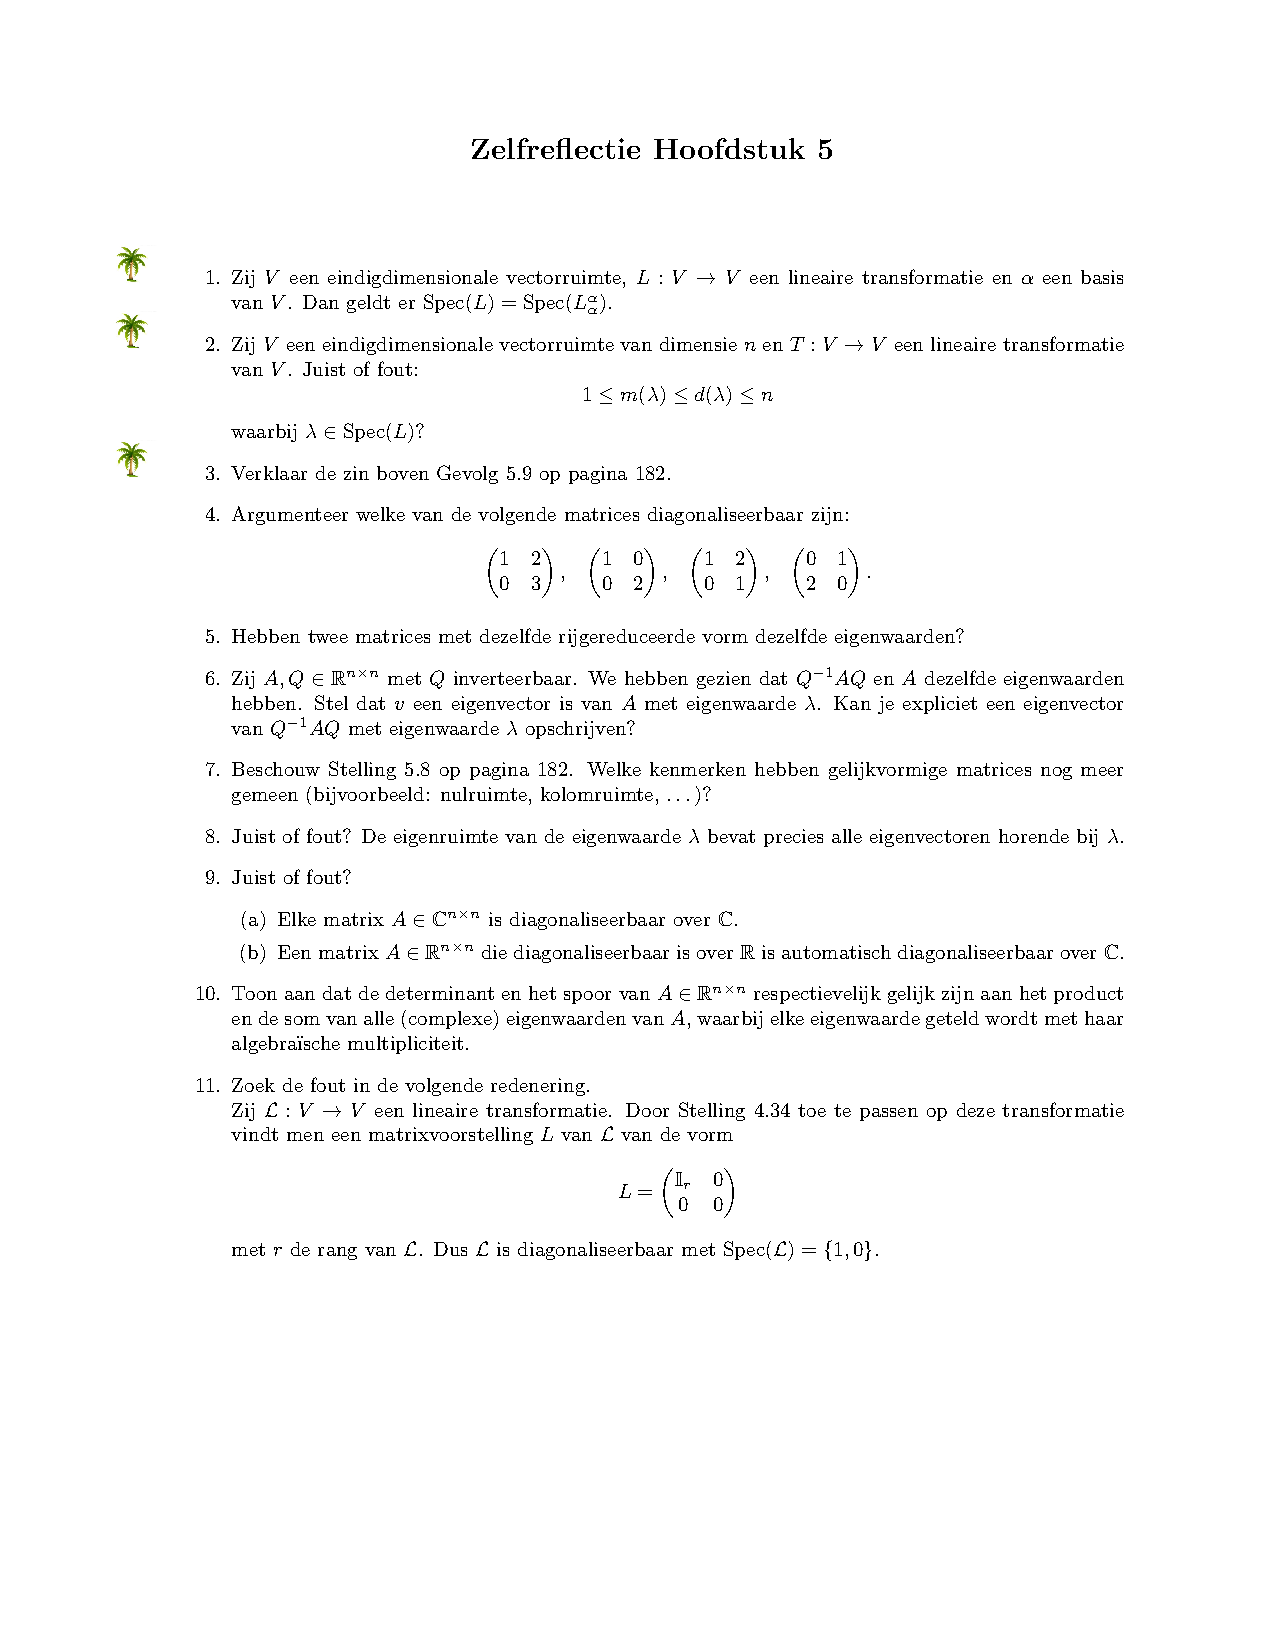
\includepdf[pages=-]{opgaven/zelfreflectie_H5.pdf}
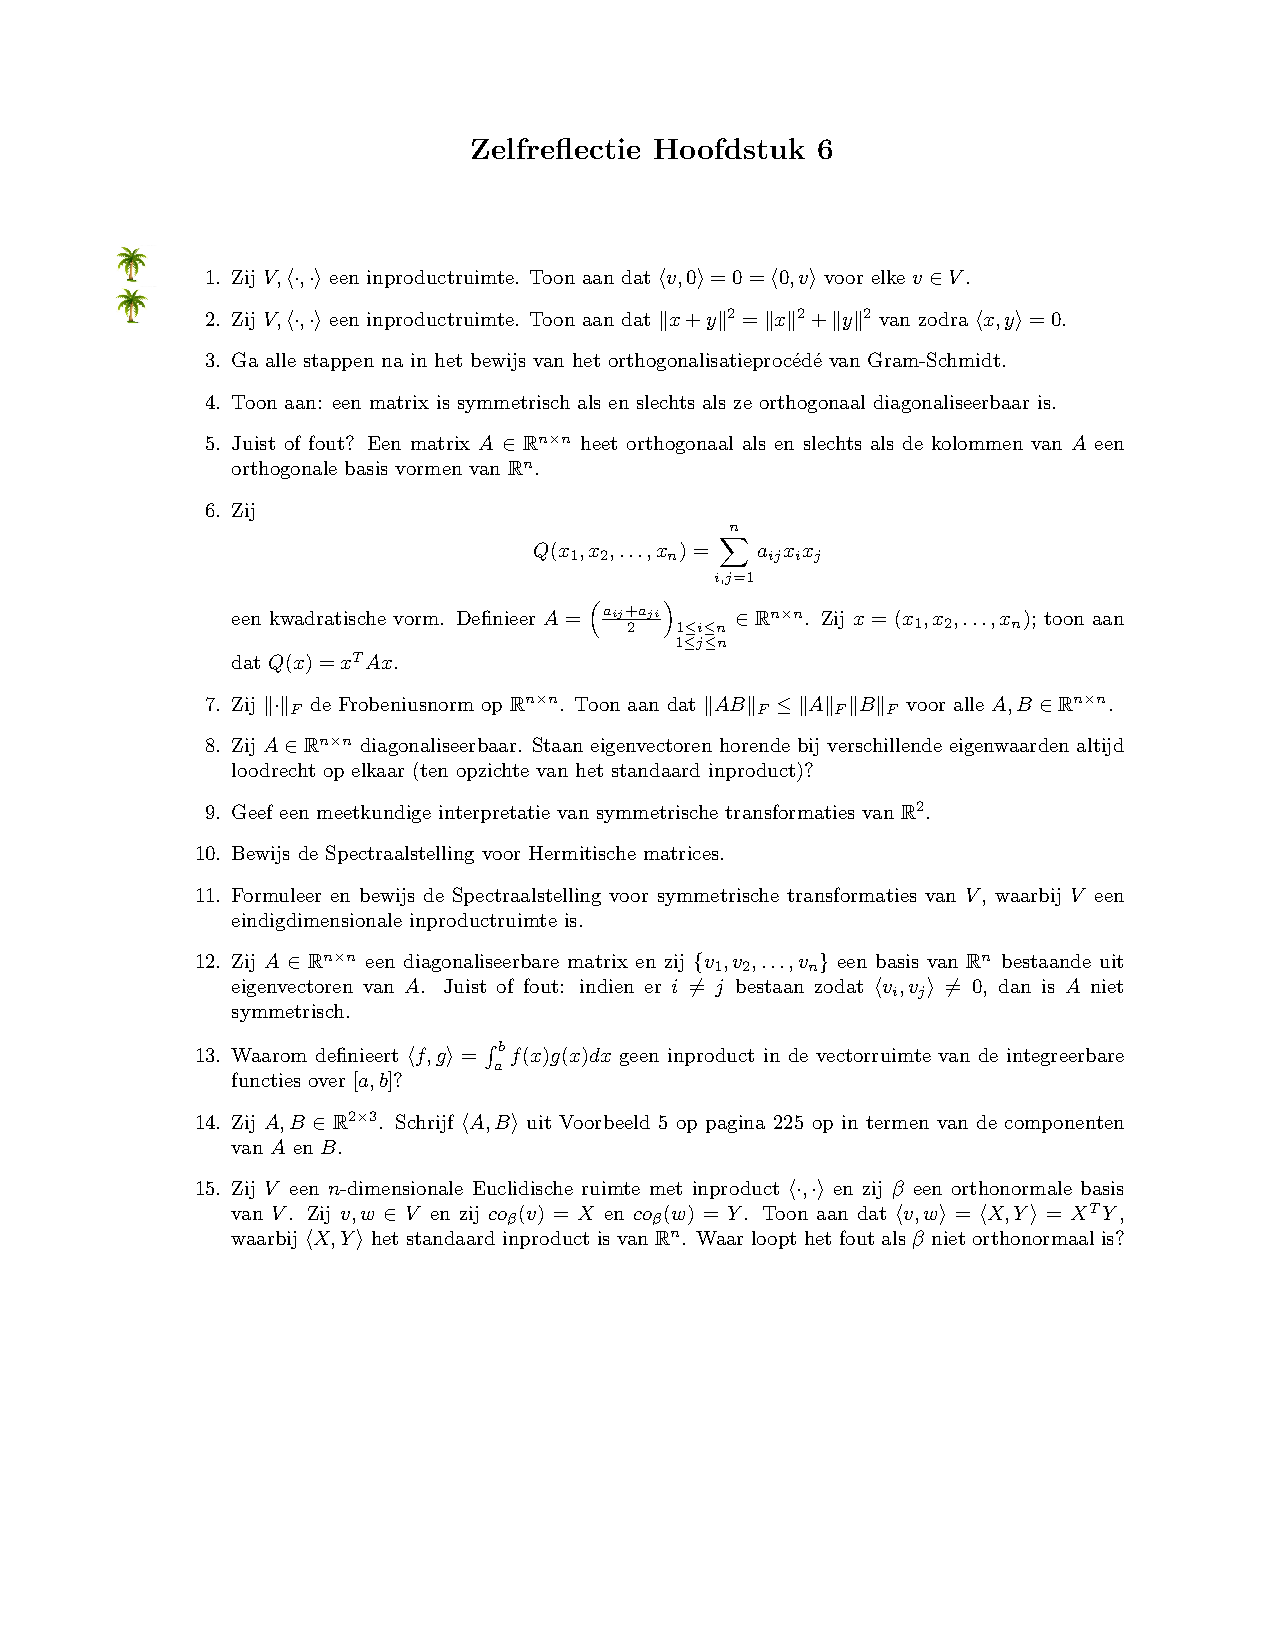
\includepdf[pages=-]{opgaven/zelfreflectie_H6.pdf}



\end{document}